
% -------------------------------------------
% Items to substitute into the ivoatex document template.
%
%\ivoagroup{Data Model Working Group}

%\title{Mango}


%\author{Laurent Michel}
    
%\author{Fran??ois Bonnarel}
    
%\author{Gilles Landais}
    
%\author{Mireille Louys}
    
%\author{Marco Molinaro}
    
%\author{Jesue Salgado}
    
%\previousversion{0.0}
      
% -------------------------------------------

\pagebreak
\section{Model: mango }
  
  % INSERT FIGURE HERE
  %\begin{figure}[h]
  %\begin{center}
  %  \includegraphics[width=\textwidth]{????.png}
  %  \caption{???}\label{fig:????}
  %\end{center}
  %\end{figure}

  Data model based oon components and data association for source data

  \subsection{AssociatedData (Abstract)}
  \label{sect:AssociatedData}
    Abstract reference to a particular dataset associated to the MANGO entity. This class is used to specify the type of the associated dataset as well as its role.

    \subsubsection{AssociatedData.semantic}
      \textbf{vodml-id: AssociatedData.semantic} \newline
      \textbf{type: \hyperref[sect:VocabularyTerm]{mango:VocabularyTerm}} \newline
      \textbf{multiplicity: 1} \newline 
      Semantic concept giving the nature of the associated data.

    \subsubsection{AssociatedData.description}
      \textbf{vodml-id: AssociatedData.description} \newline
      \textbf{type: \hyperref[sect:ivoa]{ivoa:string}} \newline
      \textbf{multiplicity: 1} \newline 
      Free text description of the associated data

  \subsection{AssociatedMangoObject}
  \label{sect:AssociatedMangoObject}
    Class holder for linking the Mango object to another \texttt{MangoObject}.

    \subsubsection{AssociatedMangoObject.mangoObject}
      \textbf{vodml-id: AssociatedMangoObject.mangoObject} \newline
      \textbf{type: \hyperref[sect:MangoObject]{mango:MangoObject}} \newline
      \textbf{multiplicity: 1} \newline 
      Reference of the associated \texttt{MangoObject}.

  \subsection{BitField}
  \label{sect:BitField}
    Property state for which each possible value is represented by a bit, so that multiple states can be contained in the same numerical value. The values defined in the related \texttt{StatusValues} must correspond to a bit patterns. This constraint is not enforced by the model.

  \subsection{Color}
  \label{sect:Color}
    Property that describes a color of the \texttt{MangoObject}. The color is not an intrinsic property of the MANGO object, but a value relative to two filters or energy bands.

    \subsubsection{Color.colorDef}
      \textbf{vodml-id: Color.colorDef} \newline
      \textbf{type: \hyperref[sect:ColorDef]{mango:ColorDef}} \newline
      \textbf{multiplicity: 1} \newline 
      Color definition. Can be either a difference of magnitudes or a hardness ratio.

  \subsection{ColorDef}
  \label{sect:ColorDef}
    Class holder for a color definition. This definition includes how the color is calculated (Mag or HR) and the filters on which the color is based. In case of hardness ratio, the energy bands must be modeled as instances of \texttt{photdm:PhotFilter} with a flat transfert function.

    \subsubsection{ColorDef.definition}
      \textbf{vodml-id: ColorDef.definition} \newline
      \textbf{type: \hyperref[sect:ColorDefinition]{mango:ColorDefinition}} \newline
      \textbf{multiplicity: 1} \newline 
      Attribute giving the way the color is calculated (Mag or HR).

    \subsubsection{ColorDef.high}
      \textbf{vodml-id: ColorDef.high} \newline
      \textbf{type: photdm:PhotFilter} \newline
      \textbf{multiplicity: 1} \newline 
      Reference to the \texttt{photdm:PhotFilter} corresponding the higher band of the color.

    \subsubsection{ColorDef.low}
      \textbf{vodml-id: ColorDef.low} \newline
      \textbf{type: photdm:PhotFilter} \newline
      \textbf{multiplicity: 1} \newline 
      Reference to the \texttt{photdm:PhotFilter} corresponding the lower band for that color.

  \subsection{EpochPosition}

      \begin{figure}[h]
        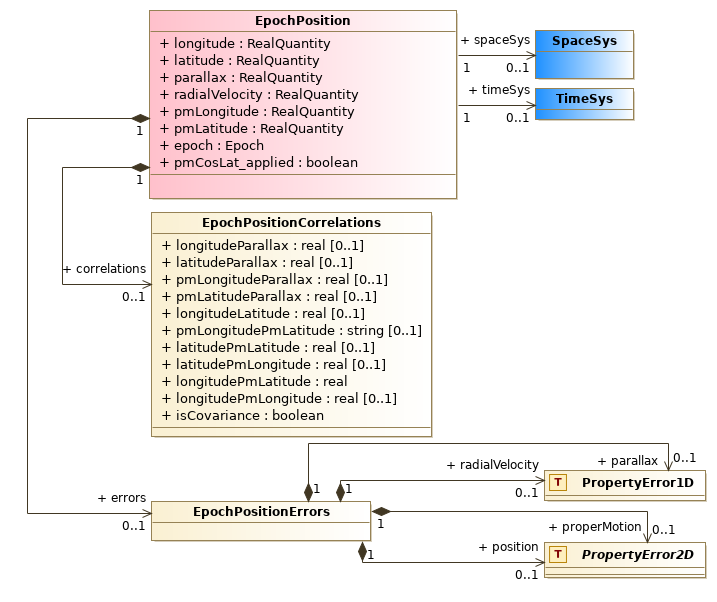
\includegraphics[width=1.0\textwidth]{../model/EpochPosition.png}
        \caption{Class EpochPosition}
        \label{fig:EpochPosition}
      \end{figure}

    
  \label{sect:EpochPosition}
    This class is a view of \texttt{Astronomical Coordinates and Coordinate Systems} components that have been put together to form a consistent description of the position of an object moving over time. It consists of a celestial position, a proper motion, a radial velocity and a parallax. All components share the same coordinate systems for both time and space coordinates. \begin{itemize} \item Both position and proper motion reuse the \texttt{coords:LonLatPoint} elements. \item The space coordinate system is imported from \texttt{coords:spaceSys}. \item The time coordinate system is imported from \texttt{coords:timeSys}. \end{itemize} The \texttt{EpochPosition} error is modeled by specific classes supporting covariance and/or correlation between components. All individual components have their own units which must be consistent to each others. This consistency is not enforced by the model.

    \subsubsection{EpochPosition.longitude}
      \textbf{vodml-id: EpochPosition.longitude} \newline
      \textbf{type: \hyperref[sect:ivoa]{ivoa:RealQuantity}} \newline
      \textbf{multiplicity: 1} \newline 
      The longitude of the Point, as a Quantity with angular units (see \texttt{coords:LonLatPoint.lon}.

    \subsubsection{EpochPosition.latitude}
      \textbf{vodml-id: EpochPosition.latitude} \newline
      \textbf{type: \hyperref[sect:ivoa]{ivoa:RealQuantity}} \newline
      \textbf{multiplicity: 1} \newline 
      The latitude of the Point, as a Quantity with angular units (see \texttt{coords:LonLatPoint.lat}.

    \subsubsection{EpochPosition.parallax}
      \textbf{vodml-id: EpochPosition.parallax} \newline
      \textbf{type: \hyperref[sect:ivoa]{ivoa:RealQuantity}} \newline
      \textbf{multiplicity: 1} \newline 
      The measured parallax in the coordinate system of the \texttt{EpochPosition} instance.

    \subsubsection{EpochPosition.radialVelocity}
      \textbf{vodml-id: EpochPosition.radialVelocity} \newline
      \textbf{type: \hyperref[sect:ivoa]{ivoa:RealQuantity}} \newline
      \textbf{multiplicity: 1} \newline 
      The measured Velocity along of the radius axis (see \texttt{meas:Velocity.coord}).

    \subsubsection{EpochPosition.pmLongitude}
      \textbf{vodml-id: EpochPosition.pmLongitude} \newline
      \textbf{type: \hyperref[sect:ivoa]{ivoa:RealQuantity}} \newline
      \textbf{multiplicity: 1} \newline 
      Velocity along the longitude axis in angular distance per unit time (see \texttt{meas:ProperMotion.coord}). The current version of the model only allows a representation in the Polar coordinate space.

    \subsubsection{EpochPosition.pmLatitude}
      \textbf{vodml-id: EpochPosition.pmLatitude} \newline
      \textbf{type: \hyperref[sect:ivoa]{ivoa:RealQuantity}} \newline
      \textbf{multiplicity: 1} \newline 
      Velocity along the latitude axis in angular distance per unit time (see \texttt{meas:ProperMotion.coord}). The current version of the model only allows a representation in the Polar coordinate space.

    \subsubsection{EpochPosition.epoch}
      \textbf{vodml-id: EpochPosition.epoch} \newline
      \textbf{type: coords:Epoch} \newline
      \textbf{multiplicity: 1} \newline 
      Position epoch expressed within the common time system (see \texttt{coords:epoch})

    \subsubsection{EpochPosition.pmCosLat\_applied}
      \textbf{vodml-id: EpochPosition.pmCosLat\_applied} \newline
      \textbf{type: \hyperref[sect:ivoa]{ivoa:boolean}} \newline
      \textbf{multiplicity: 1} \newline 
      It is common, though not universal, practice to quote longitudinal proper motion pre-multiplied by cos(latitude) so that the magnitude of the quantity is not affected by its longitudinal position. We do not constrain the value to one form or the other in this model. Instead, this flag enables providers to convey whether or not the factor has been applied (see \texttt{meas:ProperMotion.cosLat\_applied})

    \subsubsection{EpochPosition.errors}
      \textbf{vodml-id: EpochPosition.errors} \newline
      \textbf{type: \hyperref[sect:EpochPositionErrors]{mango:EpochPositionErrors}} \newline
      \textbf{multiplicity: 0..1} \newline 
      Reference to the combined errors of the \texttt{EpochPosition} components.

    \subsubsection{EpochPosition.correlations}
      \textbf{vodml-id: EpochPosition.correlations} \newline
      \textbf{type: \hyperref[sect:EpochPositionCorrelations]{mango:EpochPositionCorrelations}} \newline
      \textbf{multiplicity: 0..1} \newline 
      Reference to the correlations between the \texttt{EpochPosition} components.

    \subsubsection{EpochPosition.spaceSys}
      \textbf{vodml-id: EpochPosition.spaceSys} \newline
      \textbf{type: coords:SpaceSys} \newline
      \textbf{multiplicity: 0..1} \newline 
      System that applies the space coordinates.

    \subsubsection{EpochPosition.timeSys}
      \textbf{vodml-id: EpochPosition.timeSys} \newline
      \textbf{type: coords:TimeSys} \newline
      \textbf{multiplicity: 0..1} \newline 
      System that applies the time coordinates (the epoch).

  \subsection{EpochPositionCorrelations}
  \label{sect:EpochPositionCorrelations}
    Class holder for the correlation coefficients between the \texttt{EpochPosition} components.

    \subsubsection{EpochPositionCorrelations.positionPm}
      \textbf{vodml-id: EpochPositionCorrelations.positionPm} \newline
      \textbf{type: \hyperref[sect:correlation.Correlation22]{mango:correlation.Correlation22}} \newline
      \textbf{multiplicity: 0..1} \newline 
      Correlation matrix between the position and the proper motion.

    \subsubsection{EpochPositionCorrelations.parallaxPm}
      \textbf{vodml-id: EpochPositionCorrelations.parallaxPm} \newline
      \textbf{type: \hyperref[sect:correlation.Correlation12]{mango:correlation.Correlation12}} \newline
      \textbf{multiplicity: 0..1} \newline 
      Correlation matrix between the parallax and the proper motion.

    \subsubsection{EpochPositionCorrelations.positionParallax}
      \textbf{vodml-id: EpochPositionCorrelations.positionParallax} \newline
      \textbf{type: \hyperref[sect:correlation.Correlation21]{mango:correlation.Correlation21}} \newline
      \textbf{multiplicity: 0..1} \newline 
      Correlation matrix between the position and the parallax.

    \subsubsection{EpochPositionCorrelations.positionPosition}
      \textbf{vodml-id: EpochPositionCorrelations.positionPosition} \newline
      \textbf{type: \hyperref[sect:correlation.Correlation22]{mango:correlation.Correlation22}} \newline
      \textbf{multiplicity: 0..1} \newline 
      Self correlation matrix of the position.

    \subsubsection{EpochPositionCorrelations.properMotionPm}
      \textbf{vodml-id: EpochPositionCorrelations.properMotionPm} \newline
      \textbf{type: \hyperref[sect:correlation.Correlation22]{mango:correlation.Correlation22}} \newline
      \textbf{multiplicity: 0..1} \newline 
      Self correlation matrix of the proper motion.

  \subsection{EpochPositionErrors}
  \label{sect:EpochPositionErrors}
    Class holder for the errors of the EpochPosition attributes

    \subsubsection{EpochPositionErrors.parallax}
      \textbf{vodml-id: EpochPositionErrors.parallax} \newline
      \textbf{type: \hyperref[sect:error.PropertyError1D]{mango:error.PropertyError1D}} \newline
      \textbf{multiplicity: 0..1} \newline 
      Parallax error. This error is meant to be symmetrical

    \subsubsection{EpochPositionErrors.radialVelocity}
      \textbf{vodml-id: EpochPositionErrors.radialVelocity} \newline
      \textbf{type: \hyperref[sect:error.PropertyError1D]{mango:error.PropertyError1D}} \newline
      \textbf{multiplicity: 0..1} \newline 
      Error in the radial velocity. This error is meant to be symmetrical

    \subsubsection{EpochPositionErrors.position}
      \textbf{vodml-id: EpochPositionErrors.position} \newline
      \textbf{type: \hyperref[sect:error.PropertyError2D]{mango:error.PropertyError2D}} \newline
      \textbf{multiplicity: 0..1} \newline 
      Position error; can be an ellipse, a correlation matrix or a covariance matrix.

    \subsubsection{EpochPositionErrors.properMotion}
      \textbf{vodml-id: EpochPositionErrors.properMotion} \newline
      \textbf{type: \hyperref[sect:error.PropertyError2D]{mango:error.PropertyError2D}} \newline
      \textbf{multiplicity: 0..1} \newline 
      Position error; can be an ellipse, a correlation matrix or a covariance matrix.

  \subsection{Label}
  \label{sect:Label}
    Free text label seen as a MANGO object property.

    \subsubsection{Label.text}
      \textbf{vodml-id: Label.text} \newline
      \textbf{type: \hyperref[sect:ivoa]{ivoa:string}} \newline
      \textbf{multiplicity: 1} \newline 
      Text of label property of the MANGO object.

  \subsection{MangoObject}
  \label{sect:MangoObject}
    Central model class: applied to a data table, each row can be modelled as a MangoObject instance. Each MangoObject hosts a collection of physical or calculated parameters, a collection of associated data, a description of the data origin and an identifier.

    \subsubsection{MangoObject.identifier}
      \textbf{vodml-id: MangoObject.identifier} \newline
      \textbf{type: \hyperref[sect:ivoa]{ivoa:string}} \newline
      \textbf{multiplicity: 1} \newline 
      Unique identifier of the \texttt{MangoObject}. The uniqueness of that identifier is not managed by the model. The format is free.

    \subsubsection{MangoObject.associatedDataDock}
      \textbf{vodml-id: MangoObject.associatedDataDock} \newline
      \textbf{type: \hyperref[sect:AssociatedData]{mango:AssociatedData}} \newline
      \textbf{multiplicity: 0..*} \newline 
      Reference to the open-ended collection of all data associated with the \texttt{MangoObject}.

    \subsubsection{MangoObject.propertyDock}
      \textbf{vodml-id: MangoObject.propertyDock} \newline
      \textbf{type: \hyperref[sect:Property]{mango:Property}} \newline
      \textbf{multiplicity: 0..*} \newline 
      Reference to the open-ended collection of the \texttt{MangoObject} properties (physical or calculated).

    \subsubsection{MangoObject.dataOrigin}
      \textbf{vodml-id: MangoObject.dataOrigin} \newline
      \textbf{type: \hyperref[sect:dataorigin.DataOrigin]{mango:dataorigin.DataOrigin}} \newline
      \textbf{multiplicity: 0..1} \newline 
      Reference to the description of the origin of the \texttt{MangoObject}.

  \subsection{PhotometricProperty}
  \label{sect:PhotometricProperty}
    Observed brightness of the \texttt{MangoObject}. The distinction between fluxes and magnitudes is made by the unit. This property should refer to a photometric calibration as defined by the \texttt{PhotDM} model.

    \subsubsection{PhotometricProperty.value}
      \textbf{vodml-id: PhotometricProperty.value} \newline
      \textbf{type: \hyperref[sect:ivoa]{ivoa:RealQuantity}} \newline
      \textbf{multiplicity: 1} \newline 
      Value of the photometric property associated with a photometric calibration as defined by the \texttt{PhotDM} model.

    \subsubsection{PhotometricProperty.photCal}
      \textbf{vodml-id: PhotometricProperty.photCal} \newline
      \textbf{type: photdm:PhotCal} \newline
      \textbf{multiplicity: 1} \newline 
      Photometric calibration that applies to the photometric property. It must be an instance of \texttt{photdm:PhotCal}.

  \subsection{PhysicalProperty}
  \label{sect:PhysicalProperty}
    Place holder for any quantity that can be hold by measure as defined in the \texttt{Astronomical Measurements Model}.

    \subsubsection{PhysicalProperty.calibrationLevel}
      \textbf{vodml-id: PhysicalProperty.calibrationLevel} \newline
      \textbf{type: \hyperref[sect:CalibrationLevel]{mango:CalibrationLevel}} \newline
      \textbf{multiplicity: 1} \newline 
      Calibration level of the property (ObsCore).

    \subsubsection{PhysicalProperty.measure}
      \textbf{vodml-id: PhysicalProperty.measure} \newline
      \textbf{type: meas:Measure} \newline
      \textbf{multiplicity: 1} \newline 
      Instance of \texttt{Astronomical Measurements Model} that holds the Property value(s).

  \subsection{Property}
  \label{sect:Property}
    Class holder for a particular property, either physical or calculated, of the MANGO object. This class specifies both type and role of the property, and hosts the property instance itself.

    \noindent \textbf{constraint} \newline
    \indent    \textbf{detail: Property.One association at the time
 }\newline


    \subsubsection{Property.semantic}
      \textbf{vodml-id: Property.semantic} \newline
      \textbf{type: \hyperref[sect:VocabularyTerm]{mango:VocabularyTerm}} \newline
      \textbf{multiplicity: 1} \newline 
      Reference to a semantic concept giving the nature of the property or of the set made of the property and its associated properties.

    \subsubsection{Property.description}
      \textbf{vodml-id: Property.description} \newline
      \textbf{type: \hyperref[sect:ivoa]{ivoa:string}} \newline
      \textbf{multiplicity: 1} \newline 
      Free text description of the property or of the set made of the property and its associated properties.

    \subsubsection{Property.measure}
      \textbf{vodml-id: Property.measure} \newline
      \textbf{type: meas:Measure} \newline
      \textbf{multiplicity: 1} \newline 
      to be removed

    \subsubsection{Property.associatedProperties}
      \textbf{vodml-id: Property.associatedProperties} \newline
      \textbf{type: \hyperref[sect:Property]{mango:Property}} \newline
      \textbf{multiplicity: 1..*} \newline 
      Open-ended collection of MANGO properties associated with the \texttt{MangoObject}. These relationships are typically used to associate physical properties with time stamps and/or quality factors.

  \subsection{Shape}
  \label{sect:Shape}
    Description of the spatial extension of the MANGO object (for e.g. dust clouds).

    \subsubsection{Shape.shape}
      \textbf{vodml-id: Shape.shape} \newline
      \textbf{type: \hyperref[sect:ivoa]{ivoa:string}} \newline
      \textbf{multiplicity: 1} \newline 
      String serialization of the spatial extension of the \texttt{MangoObject}.

    \subsubsection{Shape.serialization}
      \textbf{vodml-id: Shape.serialization} \newline
      \textbf{type: \hyperref[sect:ShapeSerialization]{mango:ShapeSerialization}} \newline
      \textbf{multiplicity: 1} \newline 
      Serialization mode of the spatial extension of the MANGO entity.

    \subsubsection{Shape.spaceSys}
      \textbf{vodml-id: Shape.spaceSys} \newline
      \textbf{type: coords:SpaceSys} \newline
      \textbf{multiplicity: 0..1} \newline 
      Coordinate system that applies for the shape.

  \subsection{Status}
  \label{sect:Status}
    Property representing a status defined by a integer number that can only take on a defined number of values, each with its own description. Boolean status can be represented by \texttt{StatusValues} with 2 values e.g. 0 for False and 1 for True.

    \subsubsection{Status.status}
      \textbf{vodml-id: Status.status} \newline
      \textbf{type: \hyperref[sect:ivoa]{ivoa:integer}} \newline
      \textbf{multiplicity: 1} \newline 
      Actual value of the status.

    \subsubsection{Status.allowedValues}
      \textbf{vodml-id: Status.allowedValues} \newline
      \textbf{type: \hyperref[sect:StatusValues]{mango:StatusValues}} \newline
      \textbf{multiplicity: 0..1} \newline 
      List of the allowed values for the status. Each value has its own free text description.

  \subsection{StatusValue}
  \label{sect:StatusValue}
    Value allowed for a status, contain the value with a free text description.

    \subsubsection{StatusValue.value}
      \textbf{vodml-id: StatusValue.value} \newline
      \textbf{type: \hyperref[sect:ivoa]{ivoa:integer}} \newline
      \textbf{multiplicity: 1} \newline 
      Allowed value for a \texttt{Status}

    \subsubsection{StatusValue.description}
      \textbf{vodml-id: StatusValue.description} \newline
      \textbf{type: \hyperref[sect:ivoa]{ivoa:string}} \newline
      \textbf{multiplicity: 1} \newline 
      Free text description on the allowed value for a \texttt{Status}

  \subsection{StatusValues}
  \label{sect:StatusValues}
    Class holder for the list of the allowed values for the status.

    \subsubsection{StatusValues.values}
      \textbf{vodml-id: StatusValues.values} \newline
      \textbf{type: \hyperref[sect:StatusValue]{mango:StatusValue}} \newline
      \textbf{multiplicity: 1..*} \newline 
      List of the allowed values for the status. Each value has its own textual description.

  \subsection{VocabularyTerm}
  \label{sect:VocabularyTerm}
    Class holder for a term of a standardized vocabulary that applies to a property.

    \subsubsection{VocabularyTerm.uri}
      \textbf{vodml-id: VocabularyTerm.uri} \newline
      \textbf{type: \hyperref[sect:ivoa]{ivoa:string}} \newline
      \textbf{multiplicity: 1} \newline 
      URI the vocabulary term.

    \subsubsection{VocabularyTerm.label}
      \textbf{vodml-id: VocabularyTerm.label} \newline
      \textbf{type: \hyperref[sect:ivoa]{ivoa:string}} \newline
      \textbf{multiplicity: 1} \newline 
      Label attached to the vocabulary term. This is necessary because the URI may not contain any explicit label. This was the case for the IUA vocabulary until the Registry WG introduced rewriting rules that fix the issue.

  \subsection{WebEndpoint}
  \label{sect:WebEndpoint}
    Associated data referenced by an URL.

    \subsubsection{WebEndpoint.ContentType}
      \textbf{vodml-id: WebEndpoint.ContentType} \newline
      \textbf{type: \hyperref[sect:ivoa]{ivoa:string}} \newline
      \textbf{multiplicity: 1} \newline 
      URL mime type.

    \subsubsection{WebEndpoint.url}
      \textbf{vodml-id: WebEndpoint.url} \newline
      \textbf{type: \hyperref[sect:ivoa]{ivoa:anyURI}} \newline
      \textbf{multiplicity: 1} \newline 
      Web end-point.

  \subsection{ShapeFrame}
  \label{sect:ShapeFrame}

  Possible schemes to encode a shape in a string

  \noindent \underline{Enumeration Literals}
  \vspace{-\parsep}
  \small
  \begin{itemize}
  
    \item[\textbf{STC\_S}]: \textbf{vodml-id:} ShapeFrame.STC\_S \newline
          \textbf{description:} MOC serialization
    \item[\textbf{MOC}]: \textbf{vodml-id:} ShapeFrame.MOC \newline
          \textbf{description:} STCs serialization
  \end{itemize}
  \normalsize


  \subsection{ShapeSerialization}
  \label{sect:ShapeSerialization}

  Enumeration of the supported serialization modes for the shapes

  \noindent \underline{Enumeration Literals}
  \vspace{-\parsep}
  \small
  \begin{itemize}
  
    \item[\textbf{MOC}]: \textbf{vodml-id:} ShapeSerialization.MOC \newline
          \textbf{description:} Label indicating that the shape has been serialized as a S-MOC
    \item[\textbf{STCS}]: \textbf{vodml-id:} ShapeSerialization.STCS \newline
          \textbf{description:} Label indicating that the shape has been serialized as a STCS string
    \item[\textbf{POLYGON}]: \textbf{vodml-id:} ShapeSerialization.POLYGON \newline
          \textbf{description:} Label indicating that the shape has been serialized as a polygon (cf xtypes)
  \end{itemize}
  \normalsize


  \subsection{CalibrationLevel}
  \label{sect:CalibrationLevel}

  Enumeration of different possible calibration status of the property (Obscore)

  \noindent \underline{Enumeration Literals}
  \vspace{-\parsep}
  \small
  \begin{itemize}
  
    \item[\textbf{Raw}]: \textbf{vodml-id:} CalibrationLevel.Raw \newline
          \textbf{description:} Raw instrumental data, in a proprietary or internal data provider defined format, that needs instrument specific tools to be handled (ObsCore)
    \item[\textbf{Instrumental}]: \textbf{vodml-id:} CalibrationLevel.Instrumental \newline
          \textbf{description:} Instrumental data in a standard format which could be manipulated with standard astronomical packages (ObsCore).
    \item[\textbf{Calibrated}]: \textbf{vodml-id:} CalibrationLevel.Calibrated \newline
          \textbf{description:} Science ready data with the instrument signature removed (ObsCore)
  \end{itemize}
  \normalsize


  \subsection{ColorDefinition}
  \label{sect:ColorDefinition}

  Enumeration of the different types of colors supported by the model.

  \noindent \underline{Enumeration Literals}
  \vspace{-\parsep}
  \small
  \begin{itemize}
  
    \item[\textbf{ColorIndex}]: \textbf{vodml-id:} ColorDefinition.ColorIndex \newline
          \textbf{description:} Difference of magnitudes: typically $M_B - M_v$
    \item[\textbf{HardnessRatio}]: \textbf{vodml-id:} ColorDefinition.HardnessRatio \newline
          \textbf{description:} Normalized ratio of fluxes: $(F_{EB2} - F_{EB1}) / (F_{EB2} + F_{EB1})$
  \end{itemize}
  \normalsize


\pagebreak
\section{Package: error }
  \begin{figure}[h]
    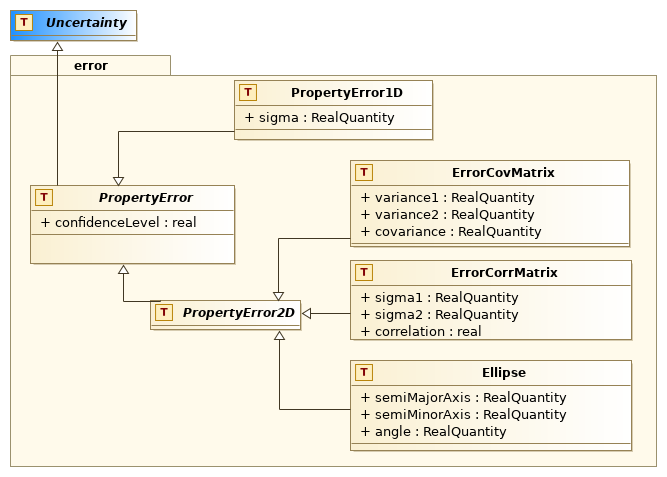
\includegraphics[width=1.0\textwidth]{../model/error.png}
    \caption{package error}
    \label{fig:error}
  \end{figure}



  % INSERT FIGURE HERE
  %\begin{figure}[h]
  %\begin{center}
  %  \includegraphics[width=\textwidth]{????.png}
  %  \caption{???}\label{fig:????}
  %\end{center}
  %\end{figure}

  The \texttt{error} package groups the MANGO built-in error classes. All these classes are derived from \texttt{meas:Uncertainty} to make them reusable by \texttt{meas:Measure} instances. Mango errors all have an attribute that specifies the confidence level

  \subsection{Ellipse}
  \label{sect:error.Ellipse}
    Elliptic error for 2D parameters such as sky positions. Major axis and minor axis have their own units, which must be the same for both. This is not enforced by the model.

    \subsubsection{Ellipse.semiMajorAxis}
      \textbf{vodml-id: error.Ellipse.semiMajorAxis} \newline
      \textbf{type: \hyperref[sect:ivoa]{ivoa:RealQuantity}} \newline
      \textbf{multiplicity: 1} \newline 
      Half of the ellipse major axis

    \subsubsection{Ellipse.semiMinorAxis}
      \textbf{vodml-id: error.Ellipse.semiMinorAxis} \newline
      \textbf{type: \hyperref[sect:ivoa]{ivoa:RealQuantity}} \newline
      \textbf{multiplicity: 1} \newline 
      Half of the ellipse minor axis

    \subsubsection{Ellipse.angle}
      \textbf{vodml-id: error.Ellipse.angle} \newline
      \textbf{type: \hyperref[sect:ivoa]{ivoa:RealQuantity}} \newline
      \textbf{multiplicity: 1} \newline 
      Angle between the North Polar Cape (NCP) and the major axis. This angle must be positive taking into account that angles are positive from North to the East. The angle has its own unit.

  \subsection{ErrorCorrMatrix}
  \label{sect:error.ErrorCorrMatrix}
    Correlation matrix for the error of a 2D quantities. The correlation matrix is symmetrical.

    \subsubsection{ErrorCorrMatrix.sigma1}
      \textbf{vodml-id: error.ErrorCorrMatrix.sigma1} \newline
      \textbf{type: \hyperref[sect:ivoa]{ivoa:RealQuantity}} \newline
      \textbf{multiplicity: 1} \newline 
      Error on the first dimension (right ascension in case of sky coordinates)

    \subsubsection{ErrorCorrMatrix.sigma2}
      \textbf{vodml-id: error.ErrorCorrMatrix.sigma2} \newline
      \textbf{type: \hyperref[sect:ivoa]{ivoa:RealQuantity}} \newline
      \textbf{multiplicity: 1} \newline 
      Error on the second dimension (declination in case of sky coordinates)

    \subsubsection{ErrorCorrMatrix.correlation}
      \textbf{vodml-id: error.ErrorCorrMatrix.correlation} \newline
      \textbf{type: \hyperref[sect:ivoa]{ivoa:real}} \newline
      \textbf{multiplicity: 1} \newline 
      Correlation coefficient between the 2 axis

  \subsection{ErrorCovMatrix}
  \label{sect:error.ErrorCovMatrix}
    Covariance matrix for the error of a 2D quantities. The covariance matrix is symmetrical.

    \subsubsection{ErrorCovMatrix.variance1}
      \textbf{vodml-id: error.ErrorCovMatrix.variance1} \newline
      \textbf{type: \hyperref[sect:ivoa]{ivoa:RealQuantity}} \newline
      \textbf{multiplicity: 1} \newline 
      Variance of the first dimension (right ascension in case of sky coordinates)

    \subsubsection{ErrorCovMatrix.variance2}
      \textbf{vodml-id: error.ErrorCovMatrix.variance2} \newline
      \textbf{type: \hyperref[sect:ivoa]{ivoa:RealQuantity}} \newline
      \textbf{multiplicity: 1} \newline 
      Variance of the second dimension (declination in case of sky coordinates)

    \subsubsection{ErrorCovMatrix.covariance}
      \textbf{vodml-id: error.ErrorCovMatrix.covariance} \newline
      \textbf{type: \hyperref[sect:ivoa]{ivoa:RealQuantity}} \newline
      \textbf{multiplicity: 1} \newline 
      Covariance of the 2 axis

  \subsection{PropertyError (Abstract)}
  \label{sect:error.PropertyError}
    Root (abstract) class of the errors that can be attached to a MANGO property. The class inherits from \texttt{meas:uncertainty} in order to be usable in the context of properties based on \texttt{Measures} classes.

    \subsubsection{PropertyError.confidenceLevel}
      \textbf{vodml-id: error.PropertyError.confidenceLevel} \newline
      \textbf{type: \hyperref[sect:ivoa]{ivoa:real}} \newline
      \textbf{multiplicity: 1} \newline 
      Confidence level of the error. The confidence level must be in $[0, 1]$ (not enforced by the VO-DML schema).

  \subsection{PropertyError1D}
  \label{sect:error.PropertyError1D}
    Symetrical error for 1D parameters

    \subsubsection{PropertyError1D.sigma}
      \textbf{vodml-id: error.PropertyError1D.sigma} \newline
      \textbf{type: \hyperref[sect:ivoa]{ivoa:RealQuantity}} \newline
      \textbf{multiplicity: 1} \newline 
      Magnitude of error on a one-dimensional parameter

  \subsection{PropertyError2D (Abstract)}
  \label{sect:error.PropertyError2D}
    Super (abstract) class for all errors of 2D parameters

\pagebreak
\section{Package: correlation }
  \begin{figure}[h]
    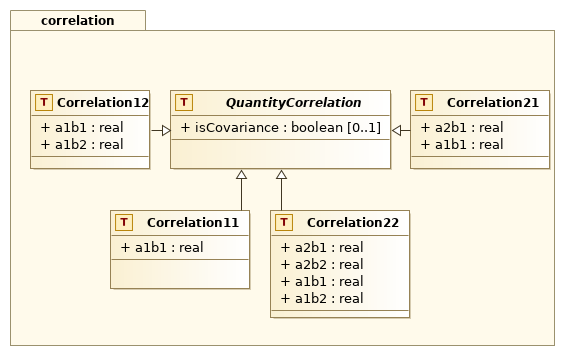
\includegraphics[width=1.0\textwidth]{../model/correlation.png}
    \caption{package correlation}
    \label{fig:correlation}
  \end{figure}



  % INSERT FIGURE HERE
  %\begin{figure}[h]
  %\begin{center}
  %  \includegraphics[width=\textwidth]{????.png}
  %  \caption{???}\label{fig:????}
  %\end{center}
  %\end{figure}

  Package grouping together all the components needed to model the correlations between property attributes.

  \subsection{Correlation11}
  \label{sect:correlation.Correlation11}
    Correlation coefficient giving the contribution of the second axis of \texttt{B} to the second axis of \texttt{A}.

    \subsubsection{Correlation11.correlation11}
      \textbf{vodml-id: correlation.Correlation11.correlation11} \newline
      \textbf{type: \hyperref[sect:ivoa]{ivoa:RealQuantity}} \newline
      \textbf{multiplicity: 1} \newline 
      Correlation coefficient giving the contribution of \texttt{B} to \texttt{A}

  \subsection{Correlation12}
  \label{sect:correlation.Correlation12}
    Correlation of a 1D property (A) with a 2D parameter (B): $A = a1b1 * B_1 + a12 * B_2$

    \subsubsection{Correlation12.correlation11}
      \textbf{vodml-id: correlation.Correlation12.correlation11} \newline
      \textbf{type: \hyperref[sect:ivoa]{ivoa:RealQuantity}} \newline
      \textbf{multiplicity: 1} \newline 
      Correlation coefficient giving the contribution of the first axis of \texttt{B} to \texttt{A}

    \subsubsection{Correlation12.correlation12}
      \textbf{vodml-id: correlation.Correlation12.correlation12} \newline
      \textbf{type: \hyperref[sect:ivoa]{ivoa:RealQuantity}} \newline
      \textbf{multiplicity: 1} \newline 
      Correlation coefficient giving the contribution of the second axis of \texttt{B} to \texttt{A}

  \subsection{Correlation21}
  \label{sect:correlation.Correlation21}
    Correlation of a 2D property (A) with a 1D parameter (B): $A_1 = a11 * B$ $A_2 = a21 * B$

    \subsubsection{Correlation21.correlation11}
      \textbf{vodml-id: correlation.Correlation21.correlation11} \newline
      \textbf{type: \hyperref[sect:ivoa]{ivoa:RealQuantity}} \newline
      \textbf{multiplicity: 1} \newline 
      Correlation coefficient giving the contribution of \texttt{B} to the first axis of \texttt{A}

    \subsubsection{Correlation21.correlation21}
      \textbf{vodml-id: correlation.Correlation21.correlation21} \newline
      \textbf{type: \hyperref[sect:ivoa]{ivoa:RealQuantity}} \newline
      \textbf{multiplicity: 1} \newline 
      Correlation coefficient giving the contribution of \texttt{B} to the second axis of \texttt{A}

  \subsection{Correlation22}
  \label{sect:correlation.Correlation22}
    Correlation of a 2D property (A) with a 2D parameter (B): $A_1 = a11 * B_1 + a12 * B_2 $ $A_2 = a21 * B_1 + a22 * B_2 $

    \subsubsection{Correlation22.sigma1}
      \textbf{vodml-id: correlation.Correlation22.sigma1} \newline
      \textbf{type: \hyperref[sect:ivoa]{ivoa:RealQuantity}} \newline
      \textbf{multiplicity: 1} \newline 
      Correlation coefficient giving the contribution of the second axis of \texttt{B} to the first axis of \texttt{A}.

    \subsubsection{Correlation22.sigma2}
      \textbf{vodml-id: correlation.Correlation22.sigma2} \newline
      \textbf{type: \hyperref[sect:ivoa]{ivoa:RealQuantity}} \newline
      \textbf{multiplicity: 1} \newline 
      Correlation coefficient giving the contribution of the second axis of \texttt{B} to the first axis of \texttt{A}.

    \subsubsection{Correlation22.correlation}
      \textbf{vodml-id: correlation.Correlation22.correlation} \newline
      \textbf{type: \hyperref[sect:ivoa]{ivoa:RealQuantity}} \newline
      \textbf{multiplicity: 1} \newline 
      Correlation coefficient giving the contribution of the second axis of \texttt{B} to the first axis of \texttt{A}.

  \subsection{QuantityCorrelation (Abstract)}
  \label{sect:correlation.QuantityCorrelation}
    Abstract type for the correlation parameters of 2 quantities

    \subsubsection{QuantityCorrelation.isCovariance}
      \textbf{vodml-id: correlation.QuantityCorrelation.isCovariance} \newline
      \textbf{type: \hyperref[sect:ivoa]{ivoa:boolean}} \newline
      \textbf{multiplicity: 0..1} \newline 
      Boolean telling whether the correlations must be interpreted as covariance or as correlation coefficients.

\pagebreak
\section{Package: dataorigin }
  \begin{figure}[h]
    \includegraphics[width=1.0\textwidth]{../model/dataorigin.png}
    \caption{package dataorigin}
    \label{fig:dataorigin}
  \end{figure}



  % INSERT FIGURE HERE
  %\begin{figure}[h]
  %\begin{center}
  %  \includegraphics[width=\textwidth]{????.png}
  %  \caption{???}\label{fig:????}
  %\end{center}
  %\end{figure}

  Package grouping together all the components needed to model the origin of \texttt{MangoObject}.

  \subsection{Article}
  \label{sect:dataorigin.Article}
    Reference article for the MANGO entity

    \subsubsection{Article.editor}
      \textbf{vodml-id: dataorigin.Article.editor} \newline
      \textbf{type: \hyperref[sect:ivoa]{ivoa:string}} \newline
      \textbf{multiplicity: 1} \newline 
      Editor name (article)

    \subsubsection{Article.article}
      \textbf{vodml-id: dataorigin.Article.article} \newline
      \textbf{type: \hyperref[sect:ivoa]{ivoa:string}} \newline
      \textbf{multiplicity: 1} \newline 
      Bibcode or DOI of the reference article

  \subsection{DataOrigin}
  \label{sect:dataorigin.DataOrigin}
    Class representing the origin of the data following the DCP note (TBD)

    \subsubsection{DataOrigin.citation}
      \textbf{vodml-id: dataorigin.DataOrigin.citation} \newline
      \textbf{type: \hyperref[sect:ivoa]{ivoa:string}} \newline
      \textbf{multiplicity: 1} \newline 
      Dataset identifier that can be used for citation (e.g. DOI)

    \subsubsection{DataOrigin.reference\_url}
      \textbf{vodml-id: dataorigin.DataOrigin.reference\_url} \newline
      \textbf{type: \hyperref[sect:ivoa]{ivoa:string}} \newline
      \textbf{multiplicity: 1} \newline 
      Dataset landing page

    \subsubsection{DataOrigin.resource\_version}
      \textbf{vodml-id: dataorigin.DataOrigin.resource\_version} \newline
      \textbf{type: \hyperref[sect:ivoa]{ivoa:string}} \newline
      \textbf{multiplicity: 1} \newline 
      Dataset version

    \subsubsection{DataOrigin.creator}
      \textbf{vodml-id: dataorigin.DataOrigin.creator} \newline
      \textbf{type: \hyperref[sect:ivoa]{ivoa:string}} \newline
      \textbf{multiplicity: 1} \newline 
      Person(s) mainly involved in the creation of the resource, generally the author

    \subsubsection{DataOrigin.cites}
      \textbf{vodml-id: dataorigin.DataOrigin.cites} \newline
      \textbf{type: \hyperref[sect:ivoa]{ivoa:string}} \newline
      \textbf{multiplicity: 1} \newline 
      Identifier (IVOID, DOI or Bibcode) of a second Resource using relation of type \texttt{cites} (\url{https://www.ivoa.net/rdf/voresource/relationship\_type/})

    \subsubsection{DataOrigin.is\_derived\_from}
      \textbf{vodml-id: dataorigin.DataOrigin.is\_derived\_from} \newline
      \textbf{type: \hyperref[sect:ivoa]{ivoa:string}} \newline
      \textbf{multiplicity: 1} \newline 
      Identifier (IVOID, DOI or Bibcode) of a second resource using relation of type \texttt{is\_derived\_from} (\url{https://www.ivoa.net/rdf/voresource/relationship\_type/})

    \subsubsection{DataOrigin.original\_date}
      \textbf{vodml-id: dataorigin.DataOrigin.original\_date} \newline
      \textbf{type: \hyperref[sect:ivoa]{ivoa:datetime}} \newline
      \textbf{multiplicity: 1} \newline 
      Date of the original resource from which the MANGO object is derived

    \subsubsection{DataOrigin.query}
      \textbf{vodml-id: dataorigin.DataOrigin.query} \newline
      \textbf{type: \hyperref[sect:dataorigin.QueryOrigin]{mango:dataorigin.QueryOrigin}} \newline
      \textbf{multiplicity: 0..1} \newline 
      Description of the request from which the data originates.

    \subsubsection{DataOrigin.rights}
      \textbf{vodml-id: dataorigin.DataOrigin.rights} \newline
      \textbf{type: \hyperref[sect:dataorigin.License]{mango:dataorigin.License}} \newline
      \textbf{multiplicity: 0..1} \newline 
      Reference to the rights that apply to the data.

    \subsubsection{DataOrigin.article}
      \textbf{vodml-id: dataorigin.DataOrigin.article} \newline
      \textbf{type: \hyperref[sect:dataorigin.Article]{mango:dataorigin.Article}} \newline
      \textbf{multiplicity: 0..1} \newline 
      Reference to the article from which the data originates.

  \subsection{License}
  \label{sect:dataorigin.License}
    Place holder for the license covering the MANGO instance

    \subsubsection{License.rights\_uri}
      \textbf{vodml-id: dataorigin.License.rights\_uri} \newline
      \textbf{type: \hyperref[sect:ivoa]{ivoa:string}} \newline
      \textbf{multiplicity: 1} \newline 
      Licence URI. Following Registry practice, this should come from SPDX https://spdx.org/licenses/, though Creative Commons URLs https://creativecommons.org are also admitted.

    \subsubsection{License.rights}
      \textbf{vodml-id: dataorigin.License.rights} \newline
      \textbf{type: \hyperref[sect:ivoa]{ivoa:string}} \newline
      \textbf{multiplicity: 1} \newline 
      License or Copyright text

  \subsection{QueryOrigin}
  \label{sect:dataorigin.QueryOrigin}
    Description of the query the MANGO instance results from.

    \subsubsection{QueryOrigin.ivoid}
      \textbf{vodml-id: dataorigin.QueryOrigin.ivoid} \newline
      \textbf{type: \hyperref[sect:ivoa]{ivoa:string}} \newline
      \textbf{multiplicity: 1} \newline 
      IVOID of the underlying data collection

    \subsubsection{QueryOrigin.publisher}
      \textbf{vodml-id: dataorigin.QueryOrigin.publisher} \newline
      \textbf{type: \hyperref[sect:ivoa]{ivoa:string}} \newline
      \textbf{multiplicity: 1} \newline 
      Data center that produced the MANGO instance

    \subsubsection{QueryOrigin.server\_software}
      \textbf{vodml-id: dataorigin.QueryOrigin.server\_software} \newline
      \textbf{type: \hyperref[sect:ivoa]{ivoa:string}} \newline
      \textbf{multiplicity: 1} \newline 
      Version of the software the produced the MANGO object instance. It is encouraged to follow \url{https://ivoa.net/documents/Notes/softid/index.html}.

    \subsubsection{QueryOrigin.service\_protocol}
      \textbf{vodml-id: dataorigin.QueryOrigin.service\_protocol} \newline
      \textbf{type: \hyperref[sect:ivoa]{ivoa:string}} \newline
      \textbf{multiplicity: 1} \newline 
      IVOID of the protocol through which the data was retrieved

    \subsubsection{QueryOrigin.request}
      \textbf{vodml-id: dataorigin.QueryOrigin.request} \newline
      \textbf{type: \hyperref[sect:ivoa]{ivoa:string}} \newline
      \textbf{multiplicity: 1} \newline 
      Full request URL including a query string. For the simple protocols,put the url-encoded form of the query parameters. For TAP queries, use the /sync UWS URL. The format is free for others request types.

    \subsubsection{QueryOrigin.query}
      \textbf{vodml-id: dataorigin.QueryOrigin.query} \newline
      \textbf{type: \hyperref[sect:ivoa]{ivoa:string}} \newline
      \textbf{multiplicity: 1} \newline 
      Input query in a formal langage such as ADQL.equest types

    \subsubsection{QueryOrigin.request\_date}
      \textbf{vodml-id: dataorigin.QueryOrigin.request\_date} \newline
      \textbf{type: \hyperref[sect:ivoa]{ivoa:datetime}} \newline
      \textbf{multiplicity: 1} \newline 
      Query execution date

    \subsubsection{QueryOrigin.contact}
      \textbf{vodml-id: dataorigin.QueryOrigin.contact} \newline
      \textbf{type: \hyperref[sect:ivoa]{ivoa:string}} \newline
      \textbf{multiplicity: 1} \newline 
      Email or URL to contact the publisher